\documentclass{beamer}
\usepackage{booktabs}
%\usepackage{amsmath}
%\usepackage{pdfpages}
%\pdfpagelayout{2 on 1}[letterpaper,border shrink=5mm]

\mode<presentation>
{
%  \usetheme{Malmoe}
\usetheme{Warsaw}
\usecolortheme{seahorse}
  % or ...

 \setbeamercovered{transparent}
  % or whatever (possibly just delete it)
 \setbeamertemplate{footline}[default]
 \setbeamertemplate{navigation symbols}{\insertslidenavigationsymbol\insertframenavigationsymbol\insertdocnavigationsymbol}
}

\title{IQC Data Summary}

%\subtitle{Include Only If Paper Has a Subtitle}

%\author{NCATS Informatics}
%\author{Dac-Trung Nguyen}
% - Give the names in the same order as the appear in the paper.
% - Use the \inst{?} command only if the authors have different
%   affiliation.

%\institute[NCATS] % (optional, but mostly needed)
%{National Center for Advancing Translational Sciences}
% - Use the \inst command only if there are several affiliations.
% - Keep it simple, no one is interested in your street address.

\date[]% (optional, should be abbreviation of conference name)
{February 18, 2013}

\begin{document}
\begin{frame}
  \titlepage
\end{frame}

\begin{frame}
\frametitle{Summary}
\begin{itemize}
\item 1,737 unique samples with experimental results 
\item 1,756 samples (of which 1,539 are unique) have been
  annotated by either Scott, Ed, or both
\item 1,102 samples for which calculated $T_\frac{1}{2} \in[0, 180]$
  minutes 
\centerline{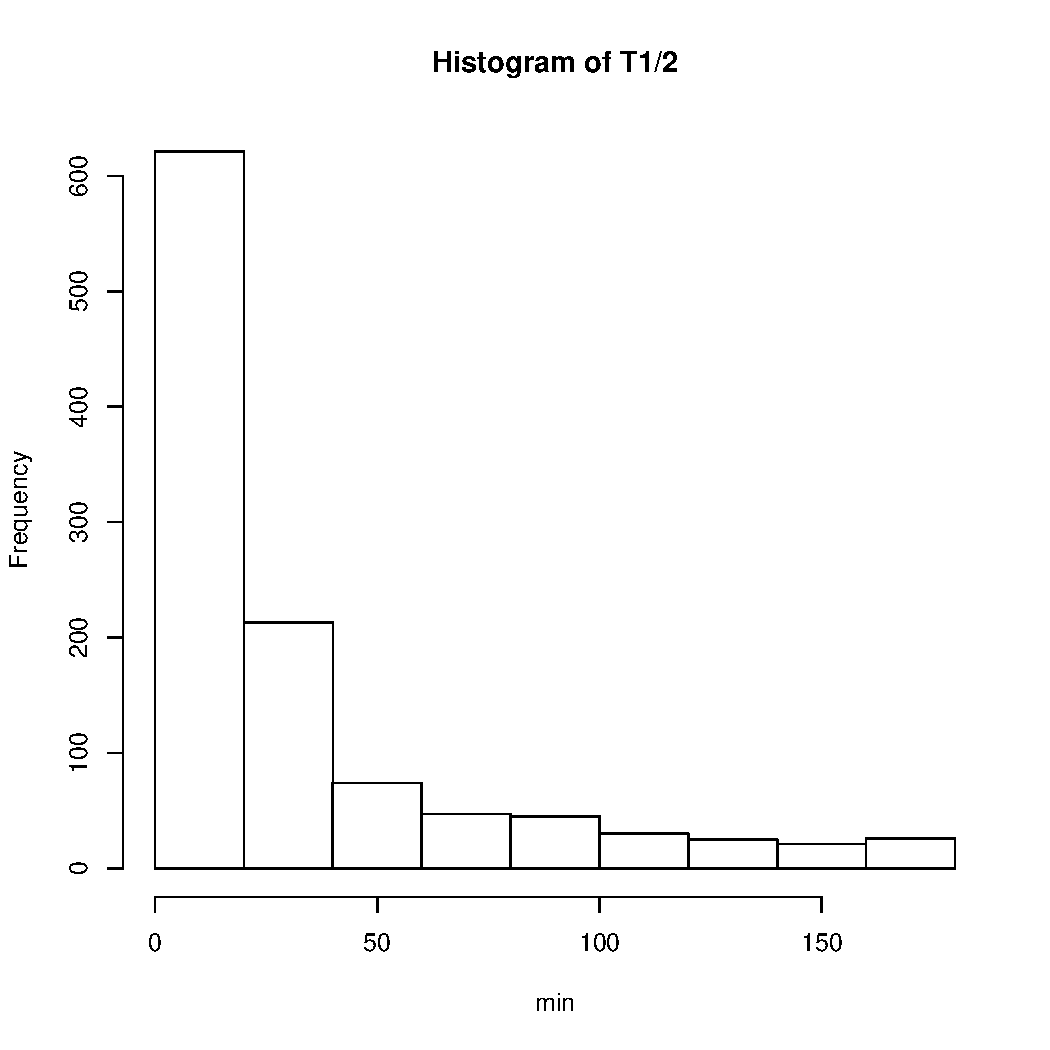
\includegraphics[height=2in]{t12}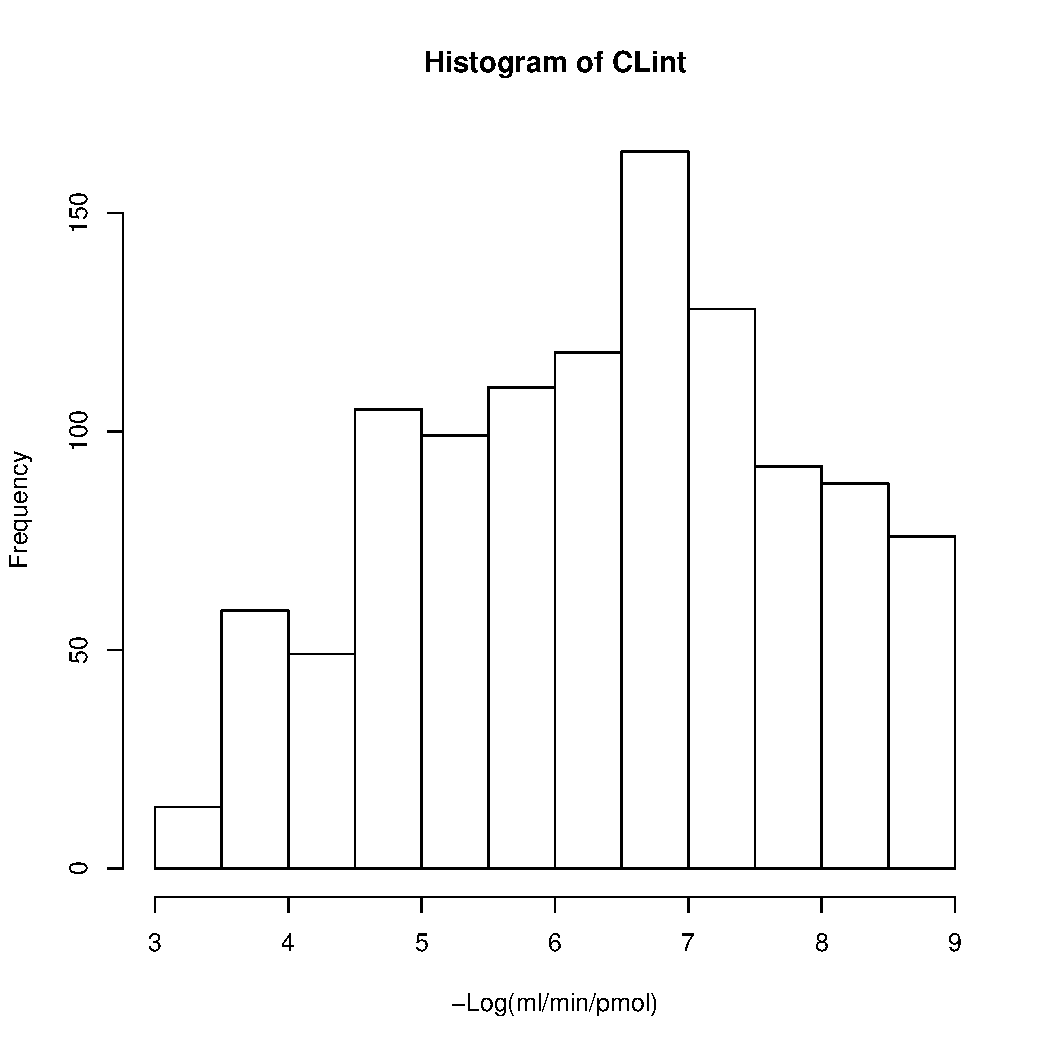
\includegraphics[height=2in]{clint}}
\end{itemize}
\end{frame}

\begin{frame}
\frametitle{Dataset}
The entire annotated
\href{https://tripod.nih.gov/share/page/site/iqc-ncats/document-details?nodeRef=workspace://SpacesStore/fafbd72e-922f-466a-94df-c599902f61bb}{\color{blue}dataset}
can be downloaded from the IQC-NCATS collaboration website at
\centerline{\href{https://tripod.nih.gov/share/}{\texttt{https://tripod.nih.gov/share/}}}.
\end{frame}
\end{document}
